\documentclass[onecolumn,aps, pre,amsmath,amssymb,longbibliography,11pt]{revtex4-2}
\usepackage{graphicx}
% \usepackage{dcolumn}
\usepackage{bm}
\usepackage{amsfonts}
\usepackage{xcolor,tabu}
\usepackage{multirow}
\usepackage{amsthm}
\usepackage{textcomp}
\usepackage{tikz}
\usepackage[colorlinks=true,
            linkcolor=blue,
            urlcolor=blue,
            citecolor=blue]{hyperref}
\hypersetup{bookmarksopen=true}
\usepackage{xr}
\usepackage{float}



\begin{document}
\title{Light attenuation of an object with arbitrary shape}

\author{Zhengyang Liu}
\date{\today}
\maketitle

\begin{figure}[h]
  \begin{center}
    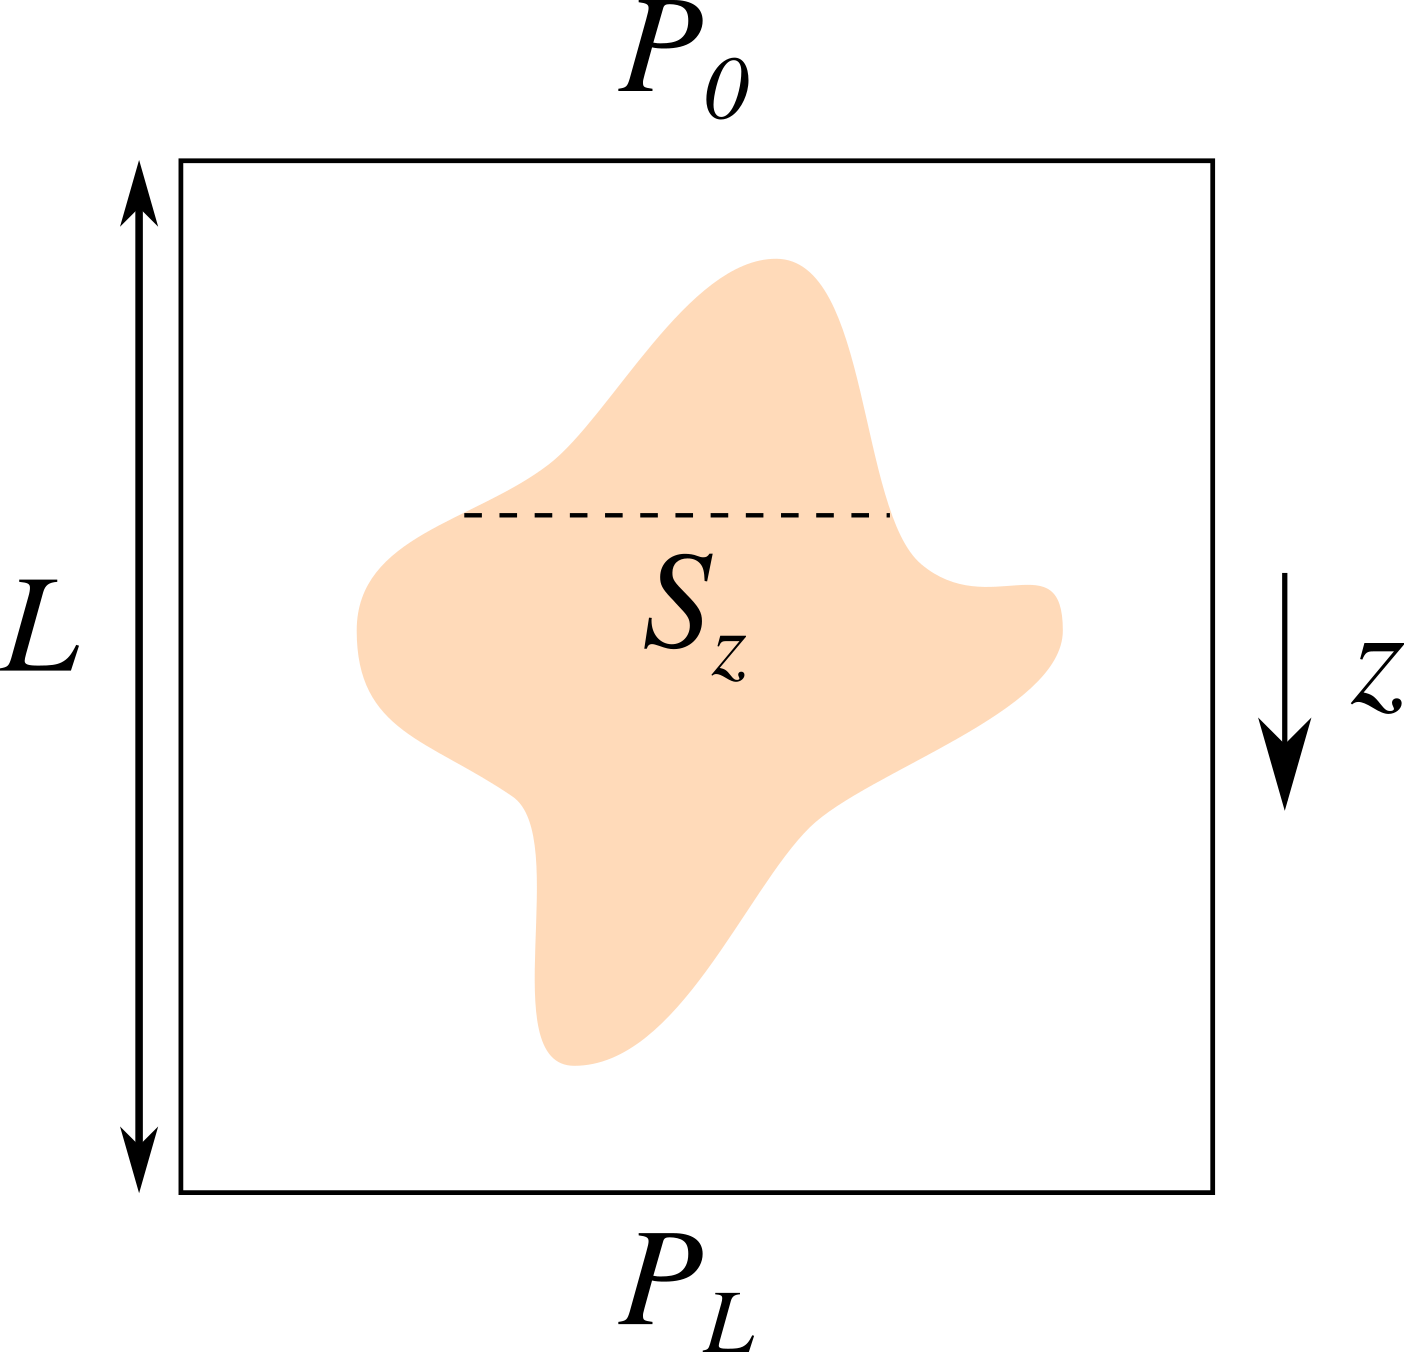
\includegraphics[width=5in]{Figures/schematic.png}
  \end{center}
\end{figure}

Consider a unit cell containing a light-absorbing object with an arbitrary shape, as shown in the schematic above. Let's assume the medium outside the object does not absorb any light (i.e. $\epsilon=0$). The incoming light has power $P_0$ on the upper surface of this cell. This light gets weaker as it propagates through the cell and ends up with power $P_L$ at the bottom of the cell. The cell has a length $L$ along the direction of the incoming light, the $z$-direction. $S_z$ denotes the cross section area of the object at position $z=z$.

We use the weak attenuation approximation of Beer's law:
$$
I = (1 - \epsilon lc) I_0
$$
where $I_0$ is the original light flux and $I$ is the attenuated light flux. Note that the power of the light is the product of flux and area.

Using this approximation, we can examine the differential power difference at position $z$.
$$
dP = -\epsilon c S_z dz
$$
Integrate over the whole cell
$$
\int_{P_0}^{P_L}dP = -\epsilon c \int_0^L S_z dz
$$
Noticing that the integral on the RHS is the volume of the object $V_{obj}$, we have
$$
P_L = P_0 - \epsilon c V_{obj}
$$

\end{document}
